\documentclass[12pt,letterpaper]{article}

\usepackage{fancyhdr}
\pagestyle{fancy}
\fancyhf{}
\rhead{Vaja 2}
\lhead{ORS}
\setlength{\headheight}{16pt}

\usepackage[utf8]{inputenc}
\usepackage[slovene]{babel}
\usepackage[colorlinks = true, urlcolor = blue]{hyperref}

\usepackage{xcolor}
\usepackage{listings}
\usepackage{graphicx}
\graphicspath{{./images/}}
\definecolor{mGreen}{rgb}{0,0.6,0}
\definecolor{mGray}{rgb}{0.5,0.5,0.5}
\definecolor{mPurple}{rgb}{0.58,0,0.82}
\definecolor{backgroundColour}{rgb}{1,1,1}

\lstdefinestyle{CStyle}{
    backgroundcolor=\color{backgroundColour},   
    commentstyle=\color{mGreen},
    keywordstyle=\color{magenta},
    numberstyle=\tiny\color{mGray},
    stringstyle=\color{mPurple},
    basicstyle=\footnotesize,
    breakatwhitespace=false,         
    breaklines=true,                 
    captionpos=b,                    
    keepspaces=true,                 
    numbers=left,                    
    numbersep=5pt,                  
    showspaces=false,                
    showstringspaces=false,
    showtabs=false,                  
    tabsize=2,
    language=C,
    frame=none
}

\begin{document}

\begin{center}
    \textbf{\Large Spoznavanje z razvojnim okoljem in delo s splošno-namenskim vhodom/izhodom}   
\end{center}

Na tokratni vaji se bomo spoznali z delom z razvojno ploščo STM32F4 in razvojnim okoljem STM32CubeIDE. Naslednjih nekaj vaj bomo prižigali LED diode in brali ali je gumb pritisnjen. Na tokratnih vajah na malo bolj naiven način, ki ga bomo nato v naslednjih tednih nadgrajevali do najbolj optimalnega pristopa, uporabe knjižnice proizvajalca mikrokrmilnika.


\section*{Vzpostavitev in nalaganje prvega projekta}

Za delo z razvojno ploščo bomo uporabljali STM32CubeIDE, ki si ga lahko brezplačno prenesete iz spletne strani podjetja ST (\href{https://www.st.com/en/development-tools/stm32cubeide.html}{povezava}). Po namestitvi zaženite program. Nov projekt za ploščo STM32F4 Discovery naredite tako, da v meniju izberete \texttt{File -> New -> STM32 Project}. Prikazal se vam bo meni za izbiranje ciljnega mikrokrmilnika. Izberite zavihek \texttt{Board Selector} in nato v desnem delu okna poiščite \texttt{STM32F4DISCOVERY}, kot je prikazano na spodnji sliki.

\begin{figure}[ht!]
  \centering
  \caption{Izbira razvojne plošče.}
  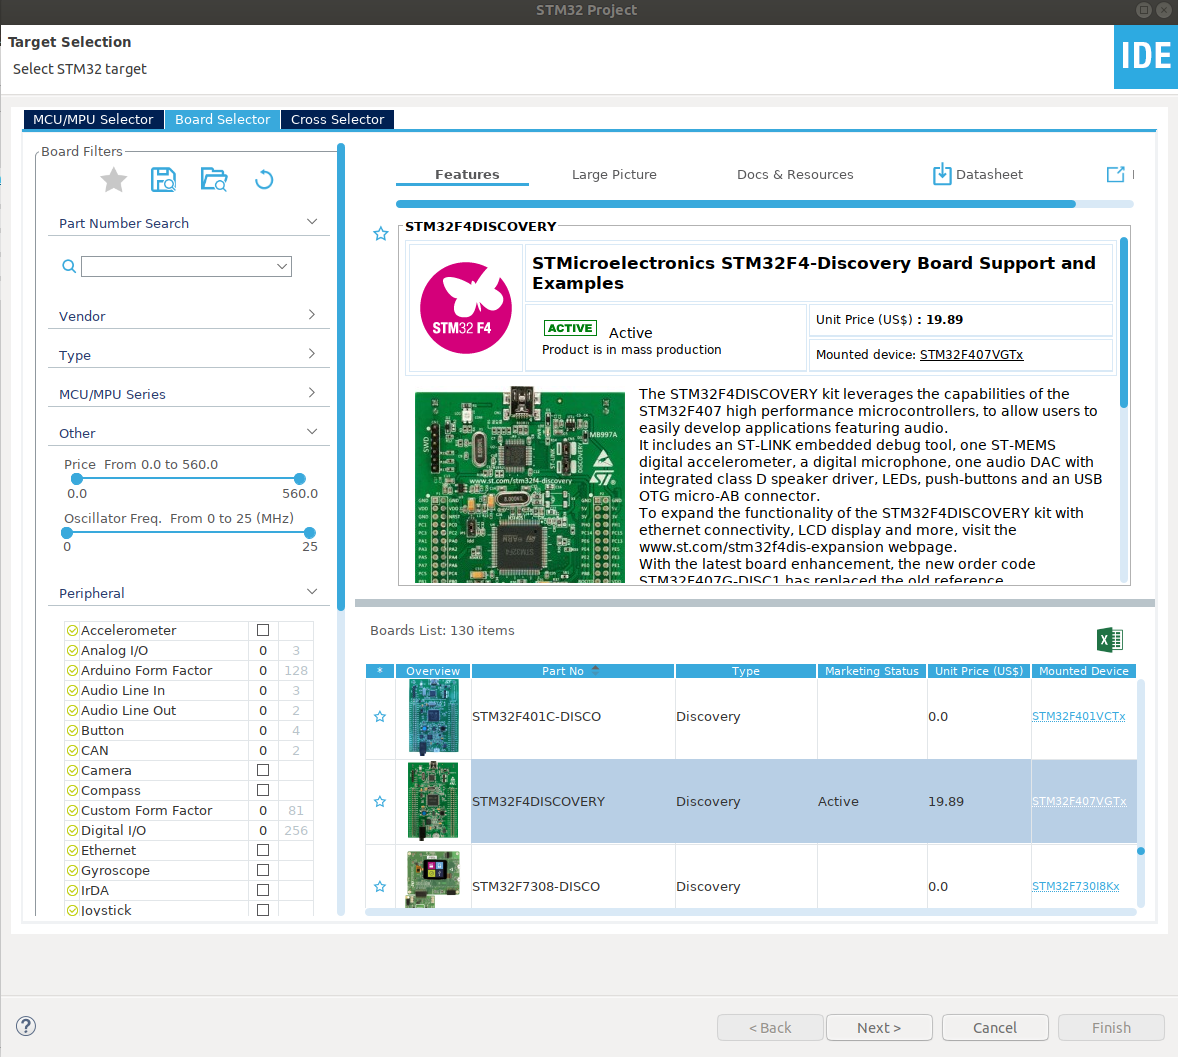
\includegraphics[width=250pt]{vaja2/izbira}
  \label{izbira}
\end{figure}

Nato kliknite \texttt{Next}, vpišite ime projekta, kliknite \texttt{Next} ter nato še \texttt{Finish}. Vse nastavitve pustite na prednastavljenih vrednostih. Na pojavno okno z vprašanjem \texttt{Initialize all peripherals with their default Mode?} odgovorite z \texttt{No}. Na ostala vprašanja pojavnih (popup) oken odgovorite pritrdilno.

V oknu \texttt{Project Explorer} odprite datoteko \texttt{Core/Src/main.c}. Ta datoteka vsebuje \texttt{main} funkcijo našega programa. Nato priključite razvojno ploščo in izberite \texttt{Run -> Debug}. V pojavnem oknu izberite \texttt{STM32 MCU CC++ Application}. Na tej točki se bo projekt prevedel. Na pojavno okno, ki vas bo vprašalo, če želite preklopiti v \texttt{Debug} perspektivo/način, odgovorite pritrdilno. V \texttt{Debug} načinu lahko program zaženete, ga ustavite, se postopoma pomikate čez program, spremljate vrednosti spremenljivk, itd.. Če želite samo zagnati vaš program kliknite na gumb \texttt{Resume} (tretji iz leve strani na sliki \ref{kontrolniGumbi}). Z gumbom \texttt{Terminate} (rdeč kvadrat na sliki \ref{kontrolniGumbi}) se vrnete nazaj v osnovno razvijalski pogled.

\begin{figure}[ht!]
  \centering
  \caption{Kontrolni gumbi.}
  
\includegraphics[width=250pt]{vaja2/kontrolni_gumbi}
  \label{kontrolniGumbi}
\end{figure}

Vso kodo, ki jo boste pisali v \texttt{main.c} datoteko pišite v dele, ki so namenjeni uporabniški kodi. Ti deli so označeni z \texttt{BEGIN} in \texttt{END} komentarjem, kot je prikazano spodaj.

\begin{center}
\begin{lstlisting}[style=CStyle]
  /* USER CODE BEGIN 1 */

  /* USER CODE END 1 */
\end{lstlisting}
\end{center}

Na ta način se boste izognili temu, da vam IDE prepiše vašo kodo ko/če boste spreminjali nastavitve projekta. Prav tako ne odstranjujte klicev funkcij \texttt{HAL\_Init()} in \texttt{SystemClock\_Config()}, ki služita osnovnim nastavitvam ravzojne plošče. Prav tako ne odstranjujte \texttt{while} zanke na koncu \texttt{main} funkcije, lahko pa poljubno spreminjate njeno vsebino. \texttt{Main} funckija se namreč na mikrokrmilniku ne sme nikoli zaključiti, saj delovanje sistema po zaključku \texttt{main} funkcije ni definirano. Tu namreč nimamo operacijskega sistema, ki bi prevzel delovanje po koncu programa.


\section*{Naiven način dela s splošno-namenskim vhodom/izhodom}

\subsection*{Branje iz naslova}

Pri Arhitekturi računalniških sistemov ste spoznali, da v zbirniku za HIP 32-bitni podatek na določenem naslov preberete z ukazom \texttt{lw r1, NASLOV (r0)}. Bolj splošna rešitev za poljuben naslov je podana spodaj. Poleg nje je zapisana tudi rešitev za isto operacijo v zbirniku za ARM procesorje. V primeru, da nas zanima 16-biten ali 8-biten podatek uporabimo ukaza \texttt{lh} in \texttt{lb}.

\begin{center}
\begin{lstlisting}[style=CStyle]
    //HIP
    lhi r1, 0x40020C00
    addui r1,r1, 0x40020C00
    lw r2, 0 (r1)
    
    //ARM
    ldr r1,=0x40020C00
    ldr r2, [r1]
\end{lstlisting}
\end{center}

V programskem jeziku C za branje iz specifičnega naslova potrebujemo kazalec. Temu kazalcu določimo naslov na katerega kaže, nato pa z derefeneciranjem (operatorjem *) preberemo vrednost na želenem naslovu. Kako bi to zapisali v primeru 32-bitne spremenljivke je prikazano spodaj.

\begin{center}
\begin{lstlisting}[style=CStyle]
    uint32_t *p = (uint32_t *) 0x40020C00;
    uint32_t vrednost = *p;
\end{lstlisting}
\end{center}

Če bi želeli brati 16-bitno ali 8-bitno vrednost, bi za to morali zgolj spremeniti tip kazalca v \texttt{uint16\_t *} ali \texttt{uint8\_t *}.

\subsection*{Pisanje na naslov}

Prav tako ste pri predmetu ARS izvedeli, da v zbirniku za HIP vrednost na določen naslov zapišemo z ukazom \texttt{sw r1, 0x400 (r0)}. Bolj splošna rešitev in rešitev za ARM je prikazana v primeru spodaj.

\begin{center}
\begin{lstlisting}[style=CStyle]
    //zelimo zapisati 0x55448000 na naslov 0x40020C18
    //HIP
    lhi r1, 0x40020C18
    addui r1,r1, 0x0C18
    lhi r2, 0x55448000
    addui r2,r2, 0x8000
    sw r2,0(r1)
    
    //ARM
    ldr r1,=0x40020C18
    ldr r2,=0x55448000
    str r2,[r1]
\end{lstlisting}
\end{center}

Za rešitev v C-ju zopet potrebujemo kazalec, ki mu določimo naslov. Za nastavljanje vrednosti na naslovu pa zopet uporabimo operator $*$, ki derefenencira kazalec. Za zapisovanje 16-bitnih ali 8-bitnih vrednosti moramo zopet zgolj spremeniti tip kazalca.

\begin{center}
\begin{lstlisting}[style=CStyle]
    uint32_t *p = (uint32_t *) 0x40020C18;
    *p = 0x55448000;
\end{lstlisting}
\end{center}


\section*{Rezervirana beseda volatile}

Rezervirano besedo \texttt{volatile} uporabimo podobno kot \texttt{unsigned}: \texttt{volatile int i = 5;}. S tem prevajalniku sporočimo, da naj ukazov s spremenljivko \texttt{i} ne optimizira. \texttt{Volatile} spremenljivke se uporabljajo kadar vemo, da se lahko vrednost spremenljivke nenadoma spremeni ali preprosto ne želimo optimizacije dela s spremenljivko. Do nenadnih sprememb spremenljivke lahko pride, če:

\begin{itemize}
    \item Je spremenljivka pomnilniško preslikana, na primer predstavlja stanje gumba.
    \item Do spremenljivke dostopamo iz prekinitveno servisnih programov (več o tem kaj to sploh je boste spoznali čez nekaj tednov).
    \item Do spremenljivke dostopa več niti.
\end{itemize}

Izklop optimizacije za posamezno spremenljivko pa potrebujemo kadar želimo narediti preprosto zakasnitev. 

\begin{center}
\begin{lstlisting}[style=CStyle]
    int i = 5000000;
    // prevajalnik bi to zanko odstranil
    while (i--) {
    }
    i = 1000000;
    // tudi to zanko bi prevajalnik odstranil
    while (1) {
        i--;
    }
    volatile int j = 5000000;
    // ta zanka bi izvedla vseh 5000000 iteracij
    while (j--) {
    }
\end{lstlisting}
\end{center}


\section*{Naloga}

Iz učilnice naložite izhodišče za main.c datoteko vašega projekta. V datoteki realizirajte sledeče funkcije:

\begin{itemize}
    \item \texttt{button\_port\_clock\_on()}, ki 32-bitnemu podatku (registru) na naslovu 0x40023830 nastavi bit 0 na 1.
    \item \texttt{led\_port\_clock\_on()}, ki 32-bitnem registru na naslovu
    0x40023830 nastavi bit 3 na 1.
    \item \texttt{button\_init()}, ki 32-bitnima podatkoma na naslovih 0x40020000 in 0x4002000C pobriše bita 0 in 1.
    \item \texttt{led\_init()}, ki nastavi pare bitov 24-25, 26-27, 28-29, 30-31 na naslovu 0x40020C00 na vrednost 01 ter pobriše bite 24-31 na naslovih 0x40020C04, 0x40020C08 in 0x40020C0C.
    \item \texttt{led\_on(uint8\_t i)}, kjer je i vrednost od 0 do 3. V primeru, da je \texttt{i=0} 16-bitnem registru na naslovu 0x40020C18 postavi bit 12 na 1, če je \texttt{i=1} postavi bit 13, pri \texttt{i=2} postavi bit 14, pri \texttt{i=3} pa postavi bit 15. Torej funkcija postavi bit \texttt{i+12} na naslovu 0x40020C18 na 1.
    \item \texttt{led\_off(uint8\_t i)}, kjer je i vrednost od 0 do 3. V primeru, da je \texttt{i=0} 16-bitnem registru na naslovu 0x40020C1A postavi bit 12 na 1. Z vrednostmi 1 do 3 pa postavi bite 13 do 15 istega registra. 
    \item \texttt{read\_button()}, ki vrne 1, če je bit 0 16-bitnega registra na naslovu 0x40020010 1, sicer vrne 0. 
    \item \texttt{delay()}, ki naredi polsekundno pavzo (zamik) v programu. Namig: uporabite preprosto zanko z odštevanjem.
\end{itemize}

Pri realizaciji funkcij si lahko pomagate s funkcijami, ki ste jih spisali v okviru prvih vaj. Z realiziranimi funkcijami nato napišite program, ki bo ob pritisku na gumb postopoma prižge vse 4 LED diode. Najprej naj prižge LED 0, čez pol sekunde LED 1 in tako naprej dokler ne gorijo vse 4 diode. Na koncu naj se vse 4 LED ugasnejo ob ponovnem pritisku pa naj se omenjeno prižiganje LED diod ponovi.

\end{document}
